% !Mode:: "TeX:UTF-8" 
\cleardoublepage
\chapter{环境的高级用法}

\section{图}

使用 subcaption 插入子图:图 \ref{fig:subcaptionExample}:

\begin{figure}[htbp]
    \centering
        \subcaptionbox{subcaption1}{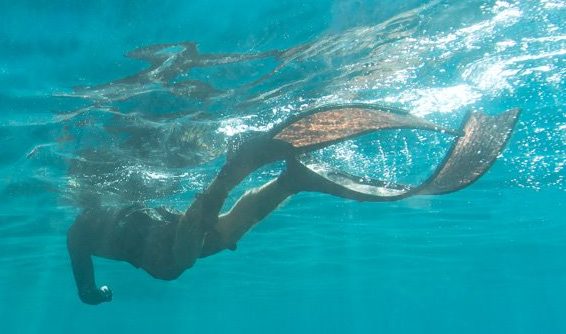
\includegraphics[width = 0.3\textwidth]{../figures/chapter2/exam1.PNG}}
        \hfill
        \subcaptionbox{subcaption2}{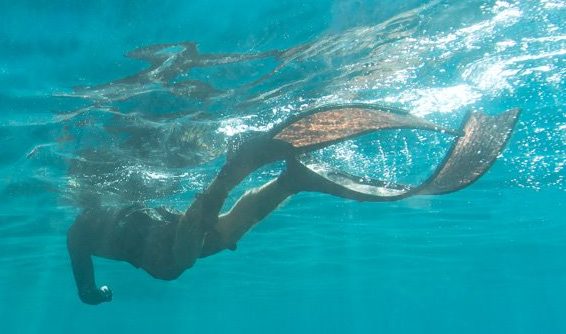
\includegraphics[width = 0.3\textwidth]{../figures/chapter2/exam1.PNG}}
        \hfill
        \subcaptionbox{subcaption3}{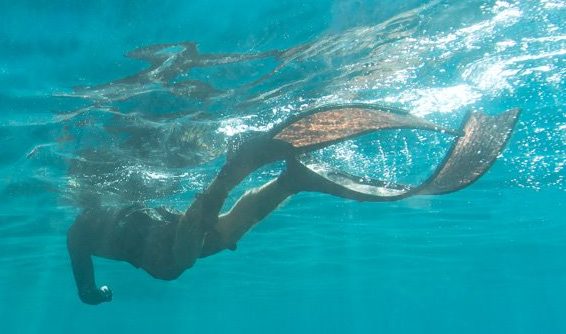
\includegraphics[width = 0.3\textwidth]{../figures/chapter2/exam1.PNG}} 
    \caption{subcaption 示例}
    \label{fig:subcaptionExample}
\end{figure}


\section{表}

\subsection{表格的辅助线}
在三线表中可以加辅助线,以适应较复杂表格的需要,如表 \ref{tbl:tableTwo} 所示。

\begin{table}[!ht]
	\renewcommand{\arraystretch}{1.2}
	\centering
	\small
	\caption{模态参数}
	\label{tbl:tableTwo}
	\begin{tabularx}{\textwidth}{c*{4}Y}
		\toprule[2pt]
		{$\textrm{方向}$}               & {$\textrm{模态阶数}$} & {$\textrm{固有频率}\,/\,\mathrm{Hz}$} & {$\textrm{阻尼比}\,/\,\mathrm{\%}$} & {$\textrm{模态刚度}\,/\,\mathrm{N\cdot m^{-1}}$} \\
		\midrule[0.5pt]
		\multirow{2}{*}{$\mathrm{X}$} & 1                 & 500                               & 2.11                             & 1.2345$\times10^7$                           \\
		                              & 2                 & 800                               & 3.11                             & 1.3579$\times10^7$                           \\
		\cmidrule[0.5pt](l){1-2}
		\multirow{2}{*}{$\mathrm{Y}$} & 1                 & 500                               & 3.11                             & 1.5432$\times10^7$                           \\
		                              & 2                 & 900                               & 5.11                             & 1.2468$\times10^7$                           \\
		\bottomrule[2pt]
	\end{tabularx}
\end{table}

\subsection{表格的横置}

使用 sidewaystable 即可

\begin{sidewaystable}[htbp]
	\renewcommand{\arraystretch}{1.2}
	\centering
	% small 不能省略
	\small
	\caption{表题也是五号字}
	\label{tbl:sidewaystableOne}
	\begin{tabularx}{\textwidth}{*{4}Y}
		\toprule[2pt]
		组号 & DOA / $^\circ$ & 带宽 / MHz & INR / dB \\
		\midrule[0.25pt]
		1  & $-30$          & 20       & 60       \\
		2  & 20             & 10       & 50       \\
		3  & 40             & 5        & 40       \\
		\bottomrule[2pt]
	\end{tabularx}
\end{sidewaystable}

\subsection{表格脚注}

\begin{table}[htbp]
	\renewcommand{\arraystretch}{1.2}
	\centering
	% small 不能省略
	\small
	\caption{表题也是五号字}
	\label{tbl:tableOneWithFootnotes}
	\begin{tabularx}{\textwidth}{*{4}Y}
		\toprule[2pt]
		组号 & DOA / $^\circ$ & 带宽 / MHz & INR / dB \\
		\midrule[0.25pt]
		1  & $-30$          & 20       & 60       \\
		2  & 20             & 10       & 50       \\
		3  & 40             & 5        & 40       \\
		\bottomrule[2pt]
	\end{tabularx}
    \begin{tablenotes}
        \item 脚注1.
        \item 脚注2.
    \end{tablenotes}
\end{table}

\section{算法}

\subsection{htbp 与 H 的区别}

htbp 会让算法位置浮动,并且行距可压缩。

H 为强制算法放在指定位置,行距不会被压缩。

\subsection{For 与 Foreach}

Foreach 可用于遍历已知集合, for 用于控制变量。

\begin{algorithm}[htbp]
    % 由于算法的行距不跟着全局设定走,所以需要在每个算法中单独设置,无论是 algothmic 还是 algorithm2e 都是这样
    \setstretch{1.28}
    \caption{For 与 Foreach 示例}
    \label{alg:forAndForeach}
    \KwIn{决策表}
    \KwOut{$AC_{max}$}
    \For{$i=1$ \KwTo $n$}{
        \ForEach{$a \in A$}{
        }
    }
    \Return{$A$}\;
\end{algorithm}

\subsection{关键字后加下横线}

去掉 format.tex 中的 \\normalem

\subsection{如何改变算法三条线粗}

我扒了两个小时源代码才知道怎么改的。

设置 package 中的
\\usepackage[linesnumbered,ruled,algochapter]\{algorithm2e\}
% 将线粗设置为学校三线表格式
\\setlength\{\\algoheightrule\}\{2pt\}
\\setlength\{\\algotitleheightrule\}\{0.25pt\}

\section{数学环境}

网络资料较多,略过。

\section{实验结果与分析}

\section{本章小结}
